\section{Prior work: Leveraging anisotropy for tailoring self-assembly in active systems}

The following is taken from an in-preparation manuscript. \cite{Moran_2018_unpublished}

\textbf{Relation to proposed thesis topic}: If we define information broadly as any quality of a building block that impacts the emergent behavior of a system of those particles (in this case, force direction and shape), then we can argue this work is looking at a few aspects of information in active systems.


\subsection{Background}

\subsection{Methods}

\subsection{Results}

\subsection{Next steps}


\begin{figure}[t]
\begin{center}
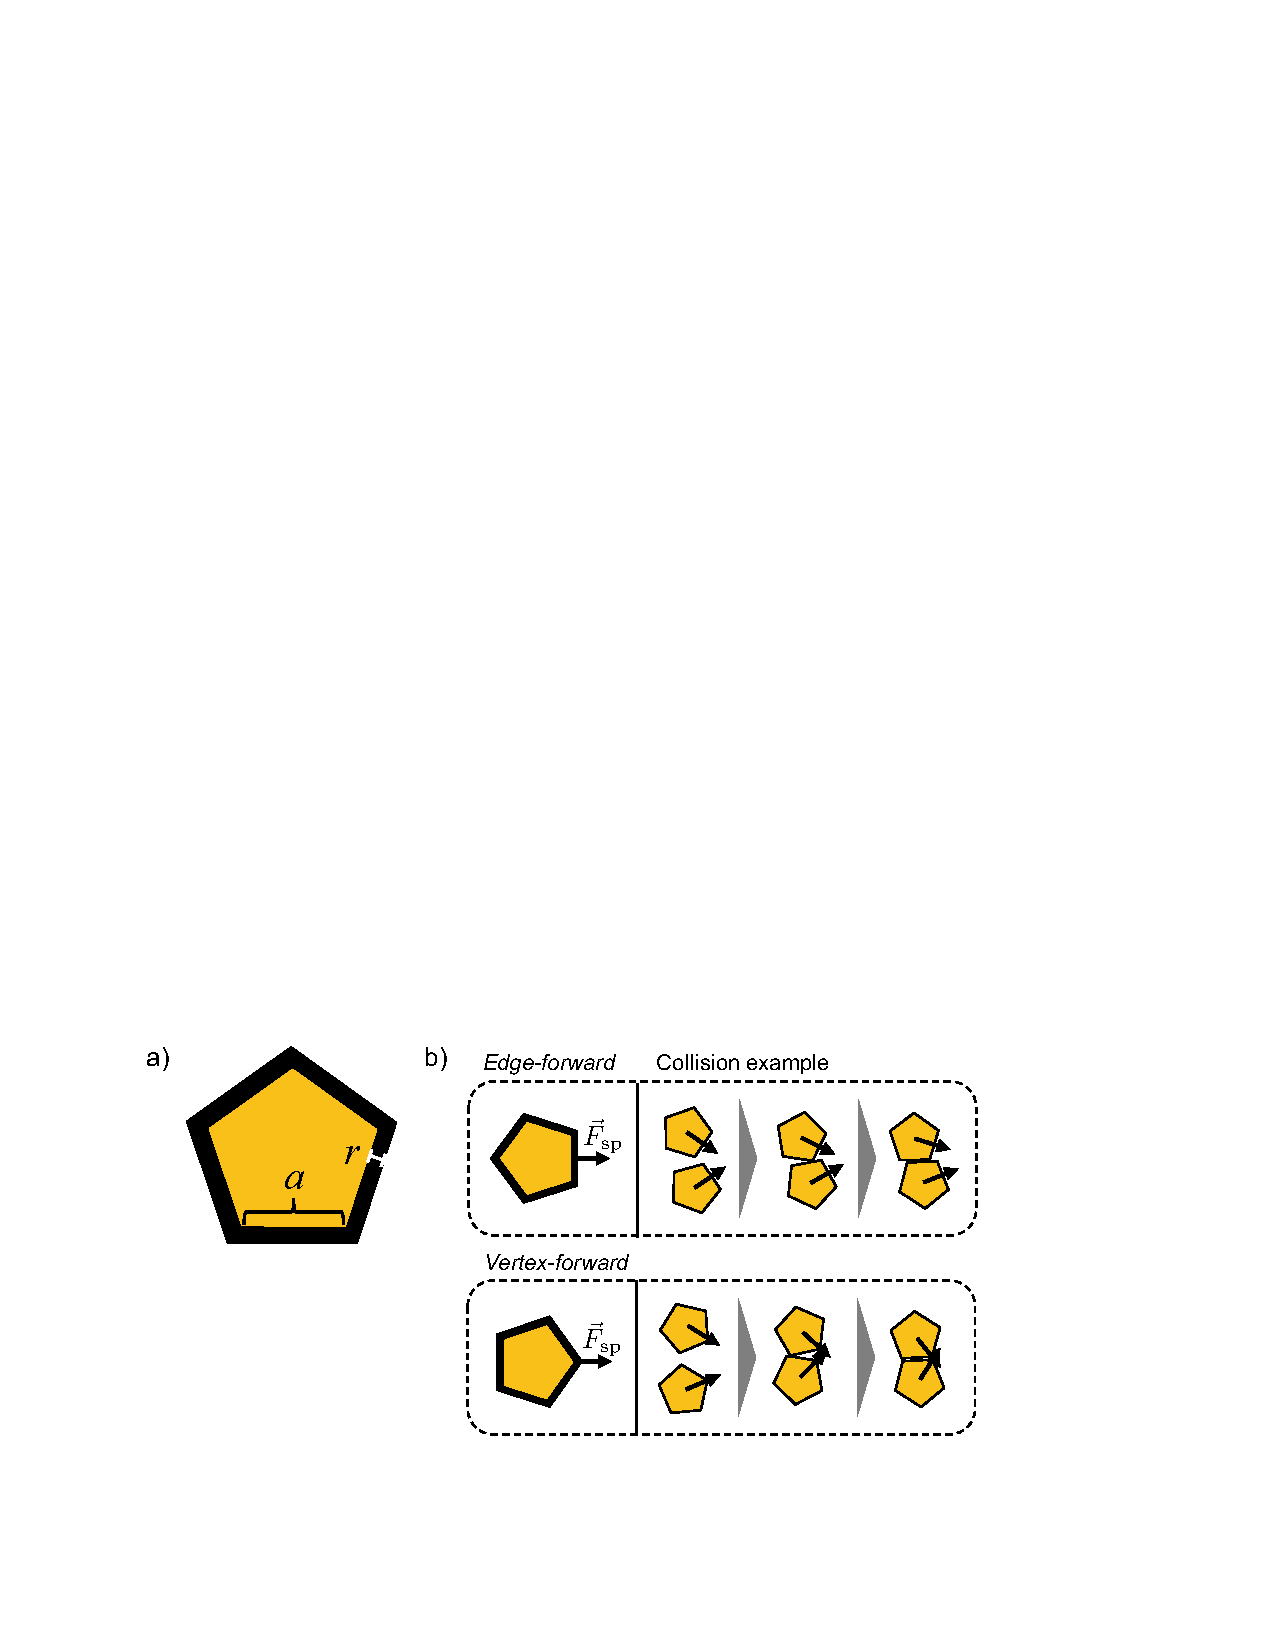
\includegraphics[width=5in]{../figures/Fig1.pdf}
\caption{\textbf{Model system}: (1) We use rounded shapes of constant S-C ratio, where the corners are rounded by a WCA potential, to ensure we can distinguish between shape steric (anisotropic) effects and isotropic behavior; (2) Force can be applied either perpendicular to the face or directed out a corner}
(Qs) should all particles be the same size?-- can't be, the way it's set up; all particles have drag of an equivalent disk; should we neglect noise? what does that mean for these simulations?
\label{fig:model}
\end{center}
\end{figure}

\begin{figure}[t]
\begin{center}
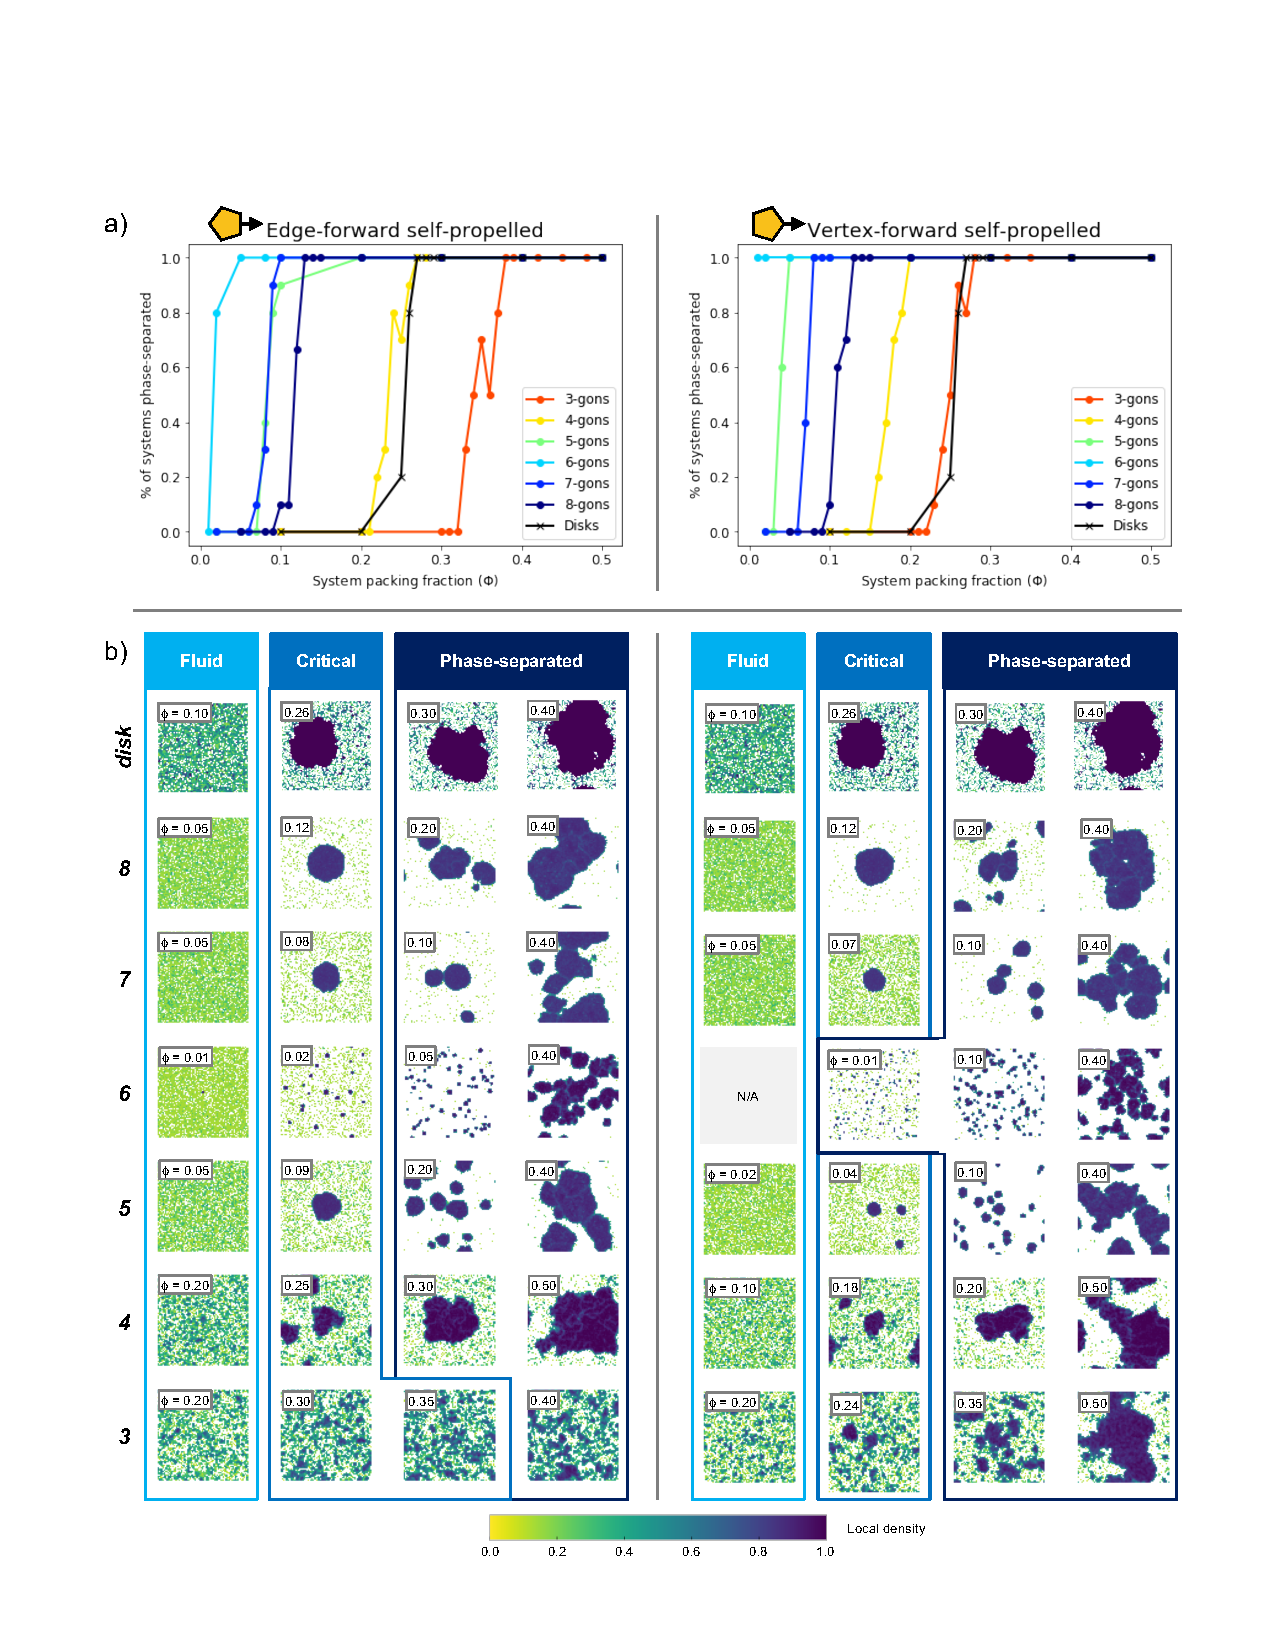
\includegraphics[width=6.5in]{../figures/Fig2.pdf}
\caption{\textbf{Critical density and nucleation behavior}: (A) Average domain size (cluster size? grain size?) versus time is different for disks versus shapes, and also depends on force director. (B) Critical density, the density at which SOME DEF OF CLUSTERING OCCURS, depends on both shape and direction of force director.}
\label{fig:phase_diagram}
\end{center}
\end{figure}

\begin{figure}[t]
\begin{center}
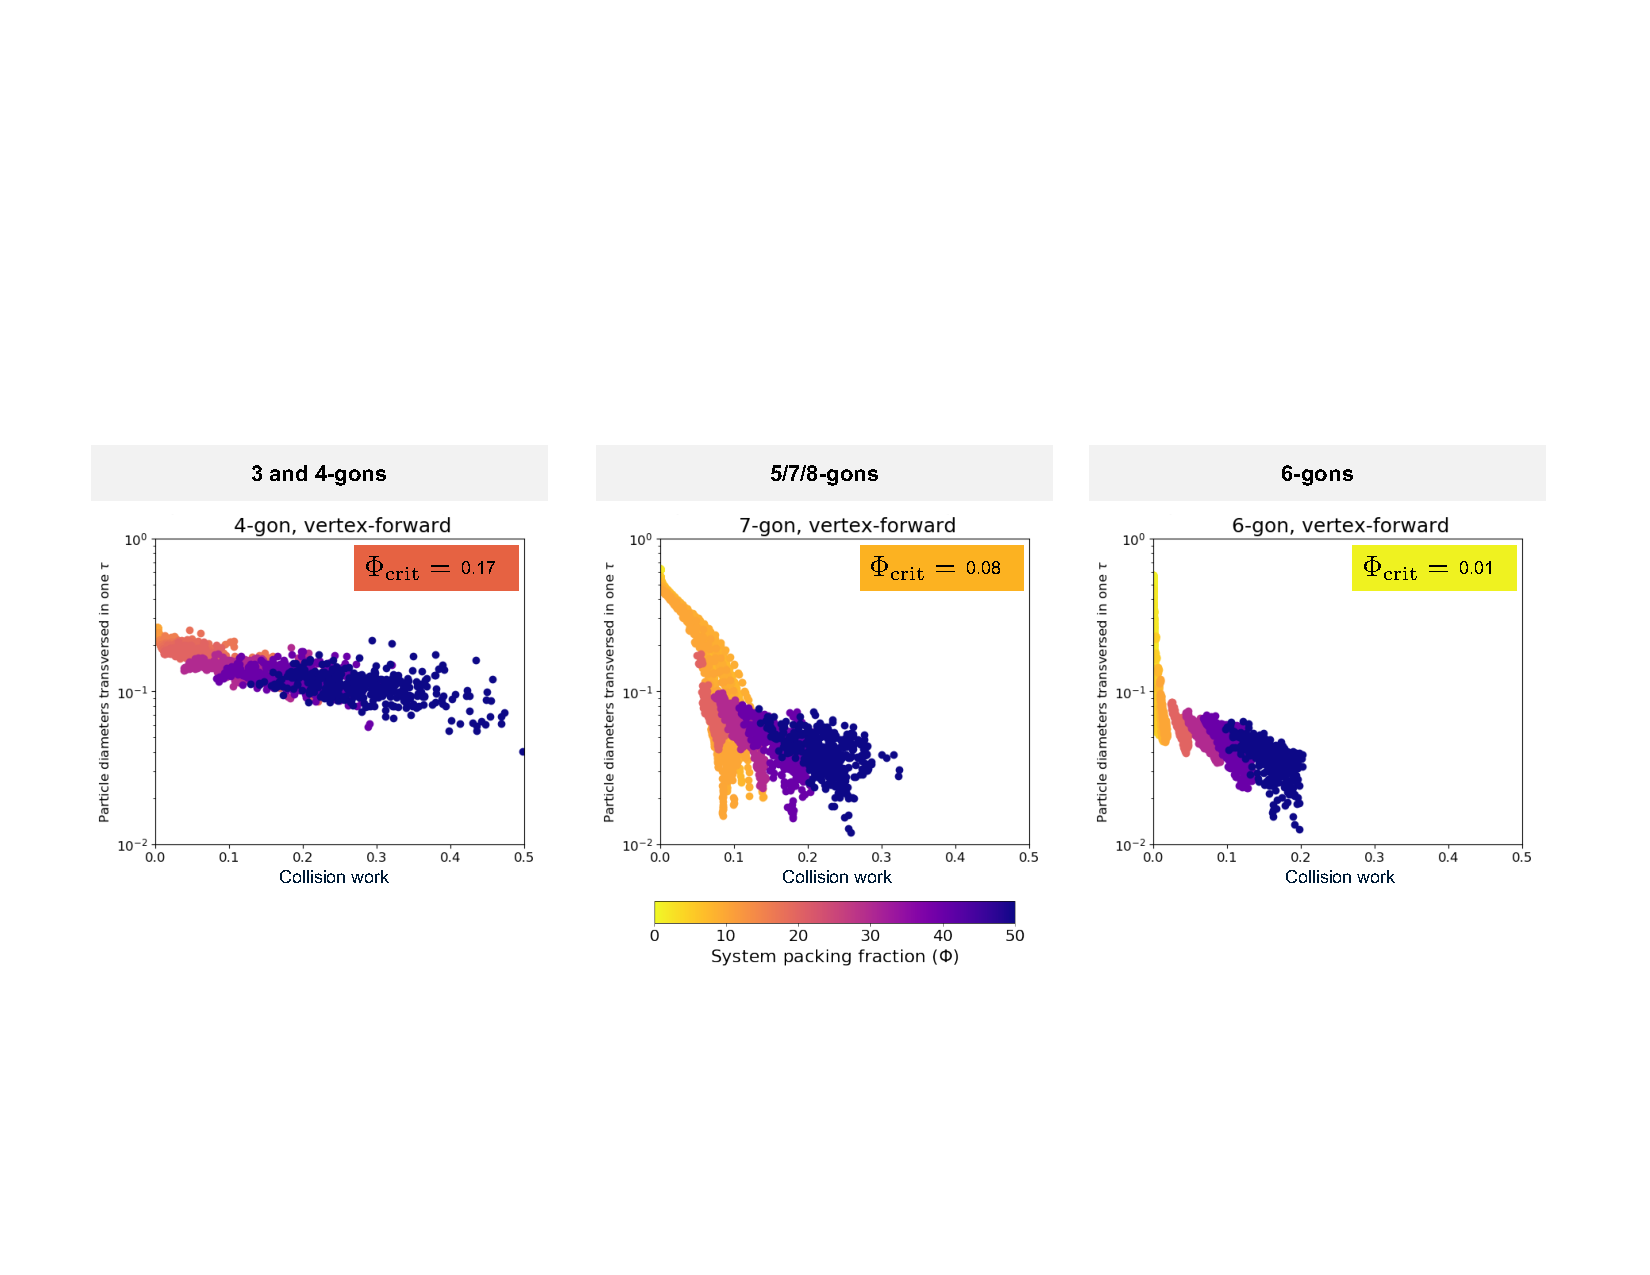
\includegraphics[width=6.5in]{../figures/Fig3.pdf}
\caption{\textbf{Collision efficiency}: Something with pressure? Not sure how to use this yet, but feel like there's something here...}
\label{fig:pressure}
\end{center}
\end{figure}


\begin{figure}[t]
\begin{center}
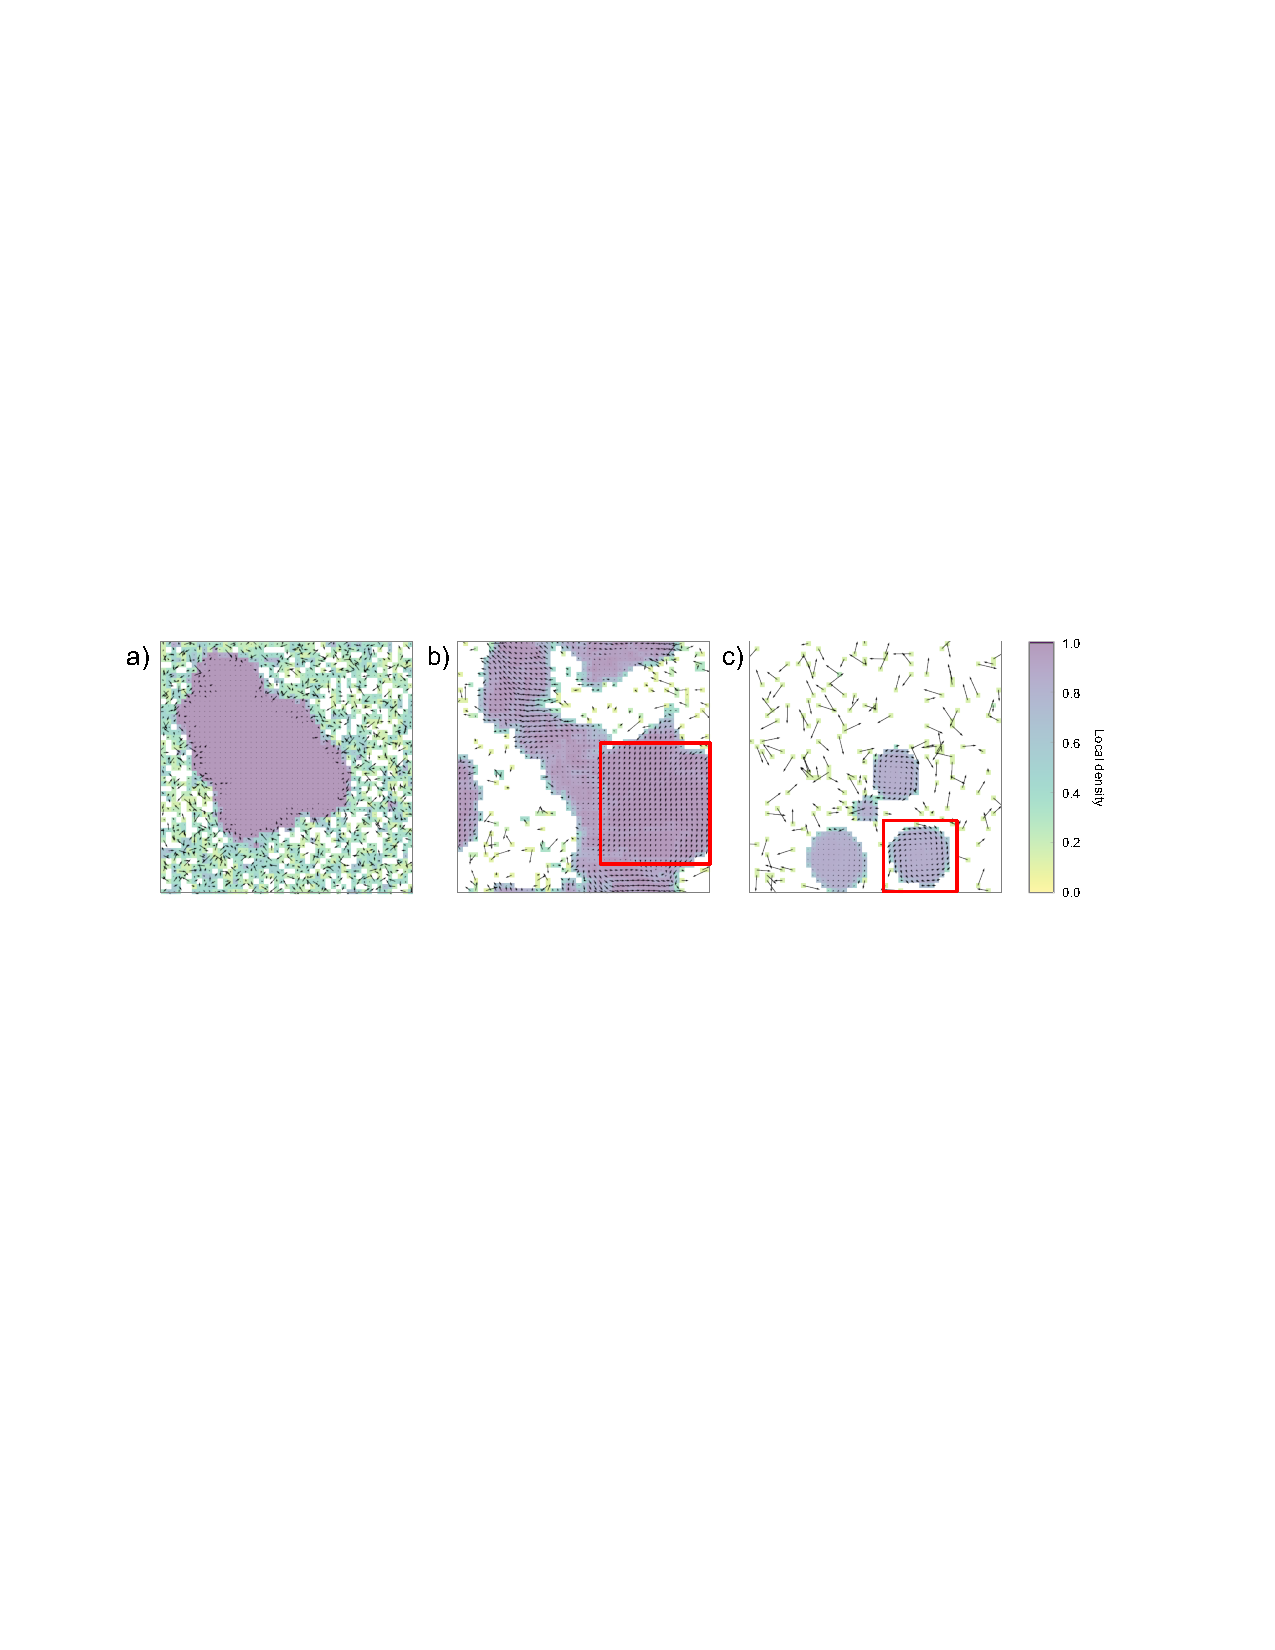
\includegraphics[width=6.5in]{../figures/Fig4.pdf}
\caption{\textbf{Displacement fields}: In contrast with disks, clusters are able to convert translational forces into rotation (highlighted in red boxes). Clusters of disks can?t sustain translational or rotational motion? clusters of shape can (this was off-hand noted in Suma et al)
}
\label{fig:velocity}
\end{center}
\end{figure}